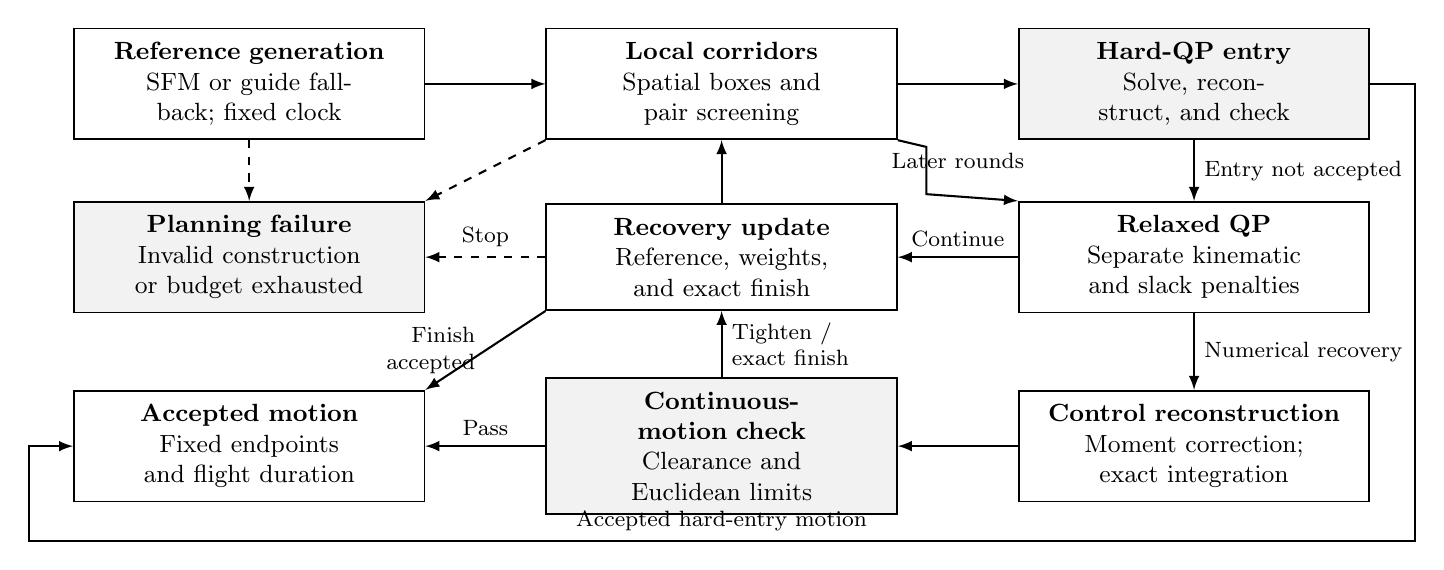
\begin{tikzpicture}[x=1cm,y=1cm,>=latex,font=\small,
 block/.style={draw=black,line width=.65pt,fill=white,text width=4.1cm,minimum height=1.05cm,inner sep=5pt,align=center},
 test/.style={block,fill=black!5},flow/.style={->,line width=.75pt}]
\node[block] (ref) at (0,0) {\textbf{Reference generation}\\SFM or guide fallback; fixed clock};
\node[block] (corr) at (6,0) {\textbf{Local corridors}\\Spatial boxes and pair screening};
\node[test] (hard) at (12,0) {\textbf{Hard-QP entry}\\Solve, reconstruct, and check};
\node[block] (soft) at (12,-2.2) {\textbf{Relaxed QP}\\Separate kinematic and slack penalties};
\node[block] (update) at (6,-2.2) {\textbf{Recovery update}\\Reference, weights, and exact finish};
\node[test] (fail) at (0,-2.2) {\textbf{Planning failure}\\Invalid construction or budget exhausted};
\node[block] (output) at (0,-4.6) {\textbf{Accepted motion}\\Fixed endpoints and flight duration};
\node[test] (check) at (6,-4.6) {\textbf{Continuous-motion check}\\Clearance and Euclidean limits};
\node[block] (control) at (12,-4.6) {\textbf{Control reconstruction}\\Moment correction; exact integration};
\draw[flow] (ref)--(corr);\draw[flow] (corr)--(hard);
\draw[flow] (hard)--node[right,font=\footnotesize]{Entry not accepted}(soft);
\draw[flow] (hard.east)--(14.8,0)--(14.8,-5.8)--node[above,font=\footnotesize]{Accepted hard-entry motion}(-2.8,-5.8)--(-2.8,-4.6)--(output.west);
\draw[flow] (soft)--node[right,font=\footnotesize]{Numerical recovery}(control);
\draw[flow] (soft.west)--node[above,font=\footnotesize]{Continue}(update.east);
\draw[flow] (update)--(corr);\draw[flow] (control)--(check);
\draw[flow] (check)--node[above,font=\footnotesize]{Pass}(output);
\draw[flow] (check)--node[right,font=\footnotesize,align=left]{Tighten /\\exact finish}(update);
\draw[flow] (update.south west)--node[left,font=\footnotesize,align=right]{Finish\\accepted}(output.north east);
\draw[flow,dashed] (ref)--(fail);\draw[flow,dashed] (corr.south west)--(fail.north east);\draw[flow,dashed] (update)--node[above,font=\footnotesize]{Stop}(fail);
\draw[flow] (corr.south east)--(8.6,-.8)--(8.6,-1.4)--(soft.north west);
\node[font=\footnotesize,anchor=south] at (9,-1.2) {Later rounds};
\end{tikzpicture}
